\section{Results}\label{sec:results}
%\textcolor{red}{Both terms graphical lasso/GLASSO being used -- one should be used.}

\subsection*{Simulation Experiments: Synthetic and Real Data}

We applied \Robocov{} on simulated multivariate normal data from three population correlation structure models (hub, Toeplitz and 1-band precision matrix) with $N$ samples, $P$ features and $\pi$ proportion of missing entries randomly distributed throughout the data matrix (Supplementary Note). Figure~\ref{fig:sim_results} shows results for all three model-settings with $N = 500, P = 50, \pi = 0.5$. In all cases, \Robocov{} generated a sparse estimate of the population correlation $\mathcal{R}$ (Section~\ref{sec:cov-estimator}) or partial correlation $\mathcal{W}$ (Section~\ref{sec:invcov-estimator}). The \Robocov{} correlation estimator captured population structure more effectively for all three models compared to the standard pairwise sample correlation estimator (Figure \ref{fig:standard_cor_sim}). The \Robocov{} partial correlation estimator also accurately captured the causal structure in the hub and 1-band precision matrix models; for the Toeplitz matrix, it recovered the high partial correlation band immediately flanking the diagonal but not the other alternating positive and negative low correlation bands (Figure \ref{fig:sim_results}). 

\begin{figure}[!tpb]
\centering
\scalebox{1}{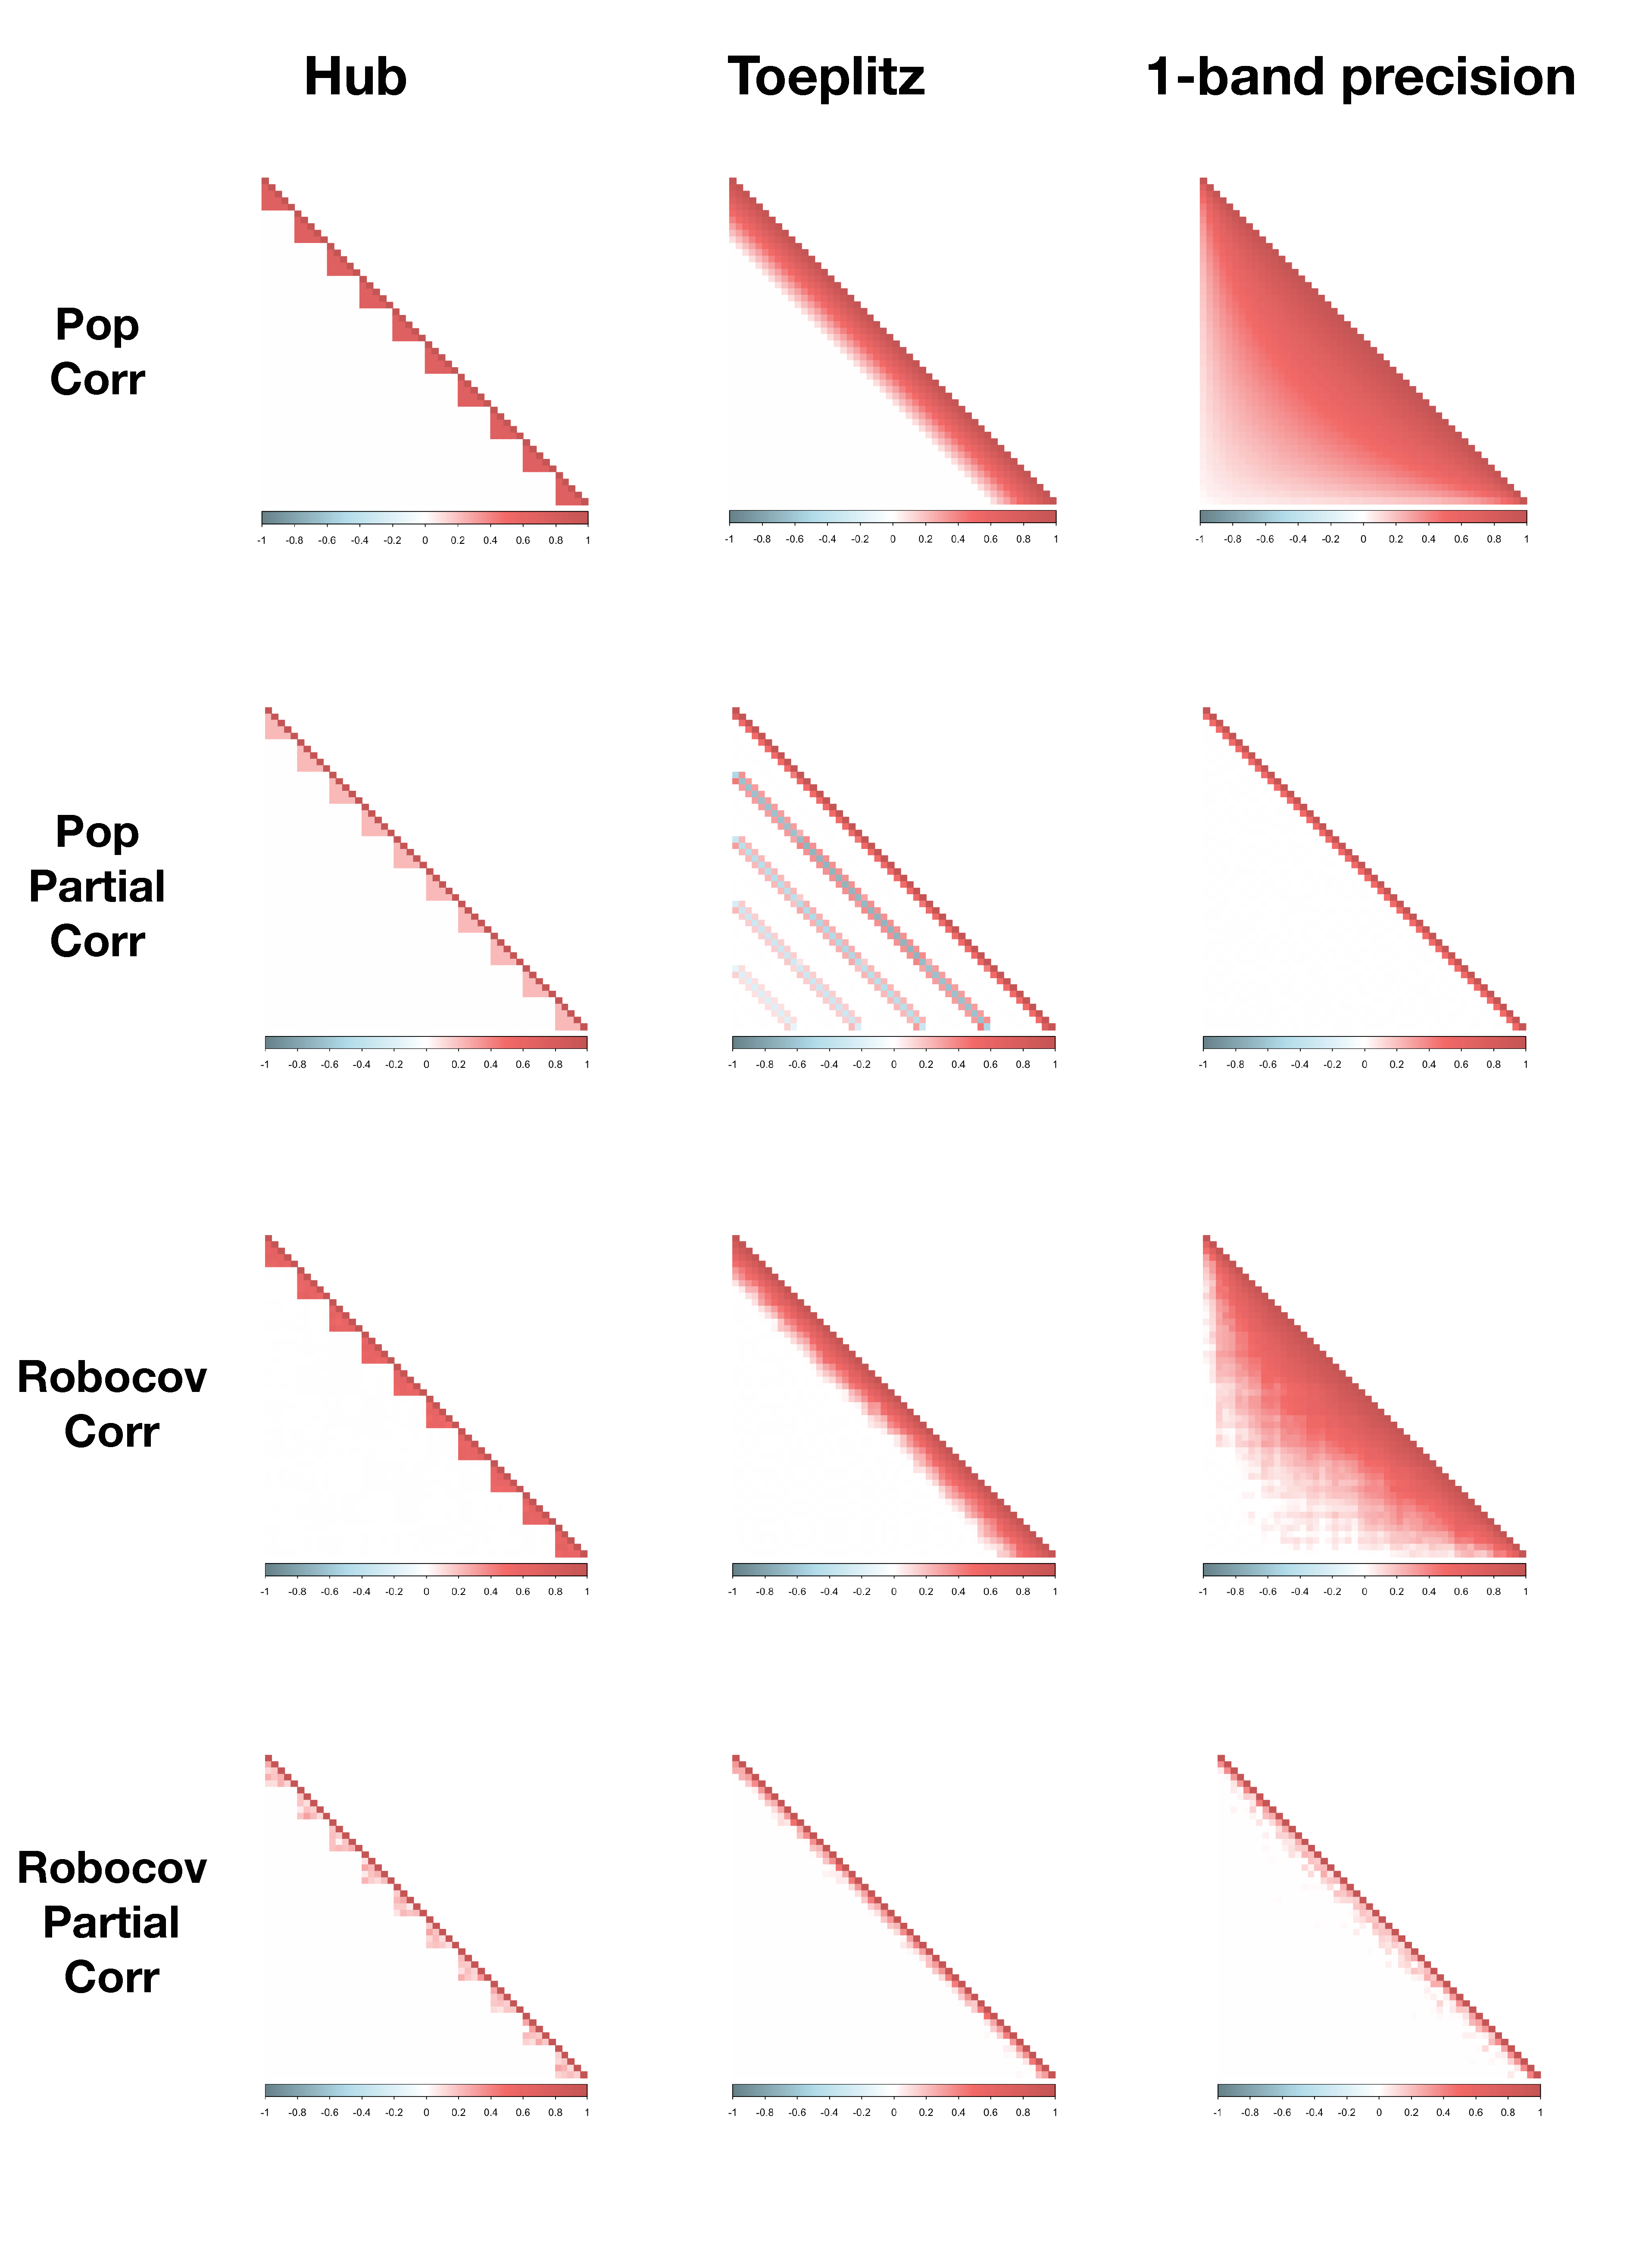
\includegraphics[width=0.5\textwidth,  trim = 0cm 5cm 0cm 0cm, clip = true  ]{Figure1_eps.eps}}
\caption{We applied \Robocov{} correlation and partial correlation estimators on data generated from Hub, Toeplitz or 1-band precision matrix based population models (Supplementary Note) with $N=500$ samples, $P=50$ features and $\pi=0.5$ proportion of missing data. We present the population correlation matrix, population partial correlation matrix, \Robocov{} correlation matrix and \Robocov{} partial correlation matrix sequentially from first to last row.}
\label{fig:sim_results}
\end{figure}

Recent work~\cite{dey2019} has shown hub-like patterns in expression correlation across tissue pairs for most genes. To this end, we applied \Robocov{} on simulated data for hub population correlation matrix structure for different settings of $N$, $P$ and $\pi$ (Supplementary Note). Two metrics of particular interest were the false positive rate (FPR) and the false negative rate (FNR) (Supplementary Note). We used these metrics to compare \Robocov{} correlation estimator with both the pairwise sample correlation estimator and  \CorShrink{}\cite{dey2019}. Across different ($N, P$, $\pi$)-settings, the \Robocov{} correlation estimator had lower FPR than \CorShrink{}. In comparison, for data with a large number of missing entries (i.e., high $\pi$), FNR for \Robocov{} was worse compared to \CorShrink{} (Table \ref{tab:tab1}). We did not compare against other shrinkage-based correlation estimators such as \textit{PDSCE}\cite{rothman2012} and \textit{corpcor}\cite{schafer2004empirical, schafer2005shrinkage} as (i) they do not account for missing entries in the data and have been shown to be sub-optimal to  \CorShrink{} for fully observed data (see Figure 4 from ref.\cite{dey2019}). 

%against estimators available from GLASSO and CLIME. Data is generated from a hub-structured population covariance matrix with different choices of $N$, $P$ and $\pi$. The three metrics are FP2 (False Positive 2-norm), FPR (False Positive Rate) and FNR (False Negative Rate). See Supplementary Note for the details of the metrics. Results are averaged over 50 replications from the same model. For all three partial correlation estimators:  \Robocov{} partial correlation, GLASSO and CLIME; the optimal sparsity inducing parameter $\lambda$ was chosen by cross-validation


\small
\begin{table}[h]
\caption{{We compare three metrics: FP2 (False Positive 2-norm), FPR (False Positive Rate) and FNR (False Negative Rate) (Supplementary Note) to compare (i) the  \Robocov{} correlation estimator (\textit{Cor}) against \CorShrink{} and the standard pairwise sample correlation estimator; and (ii) the \Robocov{} partial correlation estimator (\textit{PCor})  against estimators available from GLASSO and CLIME. Data was generated for different (N, P, $\pi$) settings and results were averaged over 50 replications from same model. Optimal $\lambda$ was chosen by cross-validation.}}
\label{tab:tab1} 
\begin{tabular}[!t]{|p{0.5cm}|p{1.1cm}|p{0.4cm}|p{0.45cm}|p{0.45cm}|p{0.4cm}|p{0.45cm}|p{0.45cm}|p{0.4cm}|p{0.45cm}|p{0.45cm}|}
\hline 
\multicolumn{11}{|c|}{Hub: N = 50, P=50} \\ \hline
& & \multicolumn{3}{c|}{$\pi$=0} & \multicolumn{3}{c|}{$\pi$=0.25} & \multicolumn{3}{c|}{$\pi$=0.5} \\ \hline
 Type & Method & FP2 & FPR & FNR &  FP2 & FPR & FNR & FP2 & FPR & FNR \\ \hline 
\multirow{ 3}{*}{Cor} & \textcolor{red}{Robocov} & 0.05 &   0 &   0  & 0.14 &   0 & 0.14 & 0.26 &   0 & 0.19 \\
& \textcolor{red}{CorShrink} & 1.4 & 0.01 &  0 & 2.2 & 0.04 & 0.03 &  4 & 0.07 & 0.09 \\
& \textcolor{red}{Standard} & 6.7 & 0.24 &  0  & 8.8 & 0.30 &  0 &  15 & 0.28 & 0 \\  \hline 
\multirow{ 3}{*}{PCor} & \textcolor{blue}{Robocov} & 0.08 & 0 & 0.07 & 0.27 & 0.01 & 0.13 & 0.47 & 0 & 0.09 \\
& \textcolor{blue}{GLASSO} & 0.12 & 0 & 0.15 & 0.29 & 0.01 & 0.15 & 0.59 & 0.02 & 0.12 \\
& \textcolor{blue}{CLIME} & 1.5 & 0.09 & 0.07 & 1.4 & 0.07 & 0.08 & 1.3 & 0.08 & 0.07 \\ \hline 
\multicolumn{11}{|c|}{Hub: N = 100, P=50} \\ \hline
& & \multicolumn{3}{c|}{$\pi$=0} & \multicolumn{3}{c|}{$\pi$=0.25} & \multicolumn{3}{c|}{$\pi$=0.5} \\ \hline
Type & Method & FP2 & FPR & FNR &  FP2 & FPR & FNR & FP2 & FPR & FNR \\ \hline
\multirow{ 3}{*}{Cor} & \textcolor{red}{Robocov} & 0.05 &   0 &   0 & 0.06 &   0 &   0 & 0.18 &   0 & 0.15\\
& \textcolor{red}{CorShrink} & 0.9 &   0 &   0 & 1.3 & 0.02 &   0 & 2.9 & 0.03 & 0.01 \\
& \textcolor{red}{Standard} & 4.8 & 0.17 &   0 & 6.2 & 0.20 &  0 &  10 & 0.31 &  0 \\ \hline 
\multirow{ 3}{*}{PCor} & \textcolor{blue}{Robocov} & 0.23 & 0 & 0.06 & 0.21 & 0 & 0.09 & 0.18 & 0.03 & 0.11 \\
& \textcolor{blue}{GLASSO} & 0.11 & 0 & 0.16 & 0.23 & 0 & 0.22 & 0.29 & 0.01 & 0.24 \\
& \textcolor{blue}{CLIME}  & 1.8 & 0.12 & 0.08 & 1.8 & 0.14 & 0.09  & 1.8 & 0.16 & 0.11 \\ \hline 
\multicolumn{11}{|c|}{Hub: N = 500, P=50} \\ \hline
& & \multicolumn{3}{c|}{$\pi$=0} & \multicolumn{3}{c|}{$\pi$=0.25} & \multicolumn{3}{c|}{$\pi$=0.5} \\ \hline
Type & Method & FP2 & FPR & FNR &  FP2 & FPR & FNR & FP2 & FPR & FNR \\ \hline
\multirow{ 3}{*}{Cor} & \textcolor{red}{Robocov}  & 0.03 &   0 &   0 & 0.01 &   0 &   0 & 0.08 &   0 &   0  \\
& \textcolor{red}{CorShrink} & 0.21 &   0 &   0 & 0.32 &   0 &   0 & 0.83 &   0 &   0\\
& \textcolor{red}{Standard} & 2.1 & 0.01 &   0 & 2.8 & 0.05 &   0 & 4.4 & 0.14 &   0 \\ \hline 
\multirow{ 3}{*}{PCor} & \textcolor{blue}{Robocov} & 0.12 & 0 & 0.11 & 0.16 & 0 & 0.12 & 0.11 & 0 & 0.14 \\
& \textcolor{blue}{GLASSO} & 0.16 & 0 & 0.19 & 0.29 & 0 & 0.20 & 0.19 & 0.02 & 0.20 \\
& \textcolor{blue}{CLIME} & 2.1 & 0.11 & 0.16 & 2.0 & 0.14 & 0.18 & 2.0 & 0.15 & 0.17 \\ \hline
\end{tabular}
\end{table}
 
\normalsize
Next, we assess the performance of the \Robocov{} partial correlation estimator for the same simulation settings (Table \ref{tab:tab1}). We are not aware of a sparse conditional graph or partial correlation estimation method that directly takes into account missing entries. Nevertheless, we compare the \Robocov{} partial correlation estimator with (i) GLASSO on the pairwise sample correlation estimator $\hat{\Sigma}$ and (ii) CLIME on an imputed data matrix where, the imputation is performed using SoftImpute~\cite{mazumder2015}. In the presence of missing data, \Robocov{} partial correlation estimator showed better FPR and FNR compared to both GLASSO and CLIME-based estimators (Table \ref{tab:tab1}). The underperformance of CLIME may be attributed to the error arising from the imputation step (Table \ref{tab:tab1}).


Next, we evaluate the predictive performance of \Robocov{} correlation estimator with pairwise sample correlation estimator and \CorShrink{}. We considered the GTEx gene expression data for an example gene (ARHGAP30) across 544 donors and 53 tissues with close to $70 \%$ missing data owing to subjects contributing only a small fraction of tissues. We split the individual by tissue data for the gene into two equal groups and  compared the estimated correlation matrix (we used different estimators: \Robocov{}, \CorShrink{} and pairwise sample correlation matrix) computed on one half of the individuals with the pairwise sample correlation matrix computed from the other half.  Both \Robocov{} and \CorShrink{} estimators considerably outperformed the pairwise sample correlation estimator, with \CorShrink{} having slightly better predictive accuracy (Figure \ref{fig:gtex_predictive} and Table \ref{tab:gtex_predictive}). As \Robocov{} and \CorShrink{} predictive performances are similar, the former may be preferable 
%in terms of interpretability.
as it results in sparse estimates, leading to better interpretability. 


An an alternative to \Robocov{}, we may consider an estimator obtained by first imputing the missing entries in the data matrix and then estimating the correlation or partial correlation matrix for the complete data. For the same ARHGAP30 gene, we performed imputation by either a low rank factorization (SoftImpute\cite{mazumder2015}, with or without scaling) or a median based approach (replacing the missing entries of a feature by the median value of the observed entries). The correlation matrix obtained by SoftImpute (both  with and without scaling) showed artificial high negative and positive correlation sweeps between brain and non-brain tissues that were not observed in the pairwise correlation matrix (Figure \ref{fig:supp_imputed}). One possible explanation of this is that the data matrices in our case do not seem to have a low rank representation based on eigenvalue analysis (Figure \ref{fig:gtex_highrank}).  The median based imputation method on the other hand, is prone to showing false positives---for example, we see a high correlation between Fallopian tube and Cervix-Ectocervix, which is a consequence of only 3 individuals contributing  both the tissues (Figure \ref{fig:supp_imputed}). \Robocov{} can effectively get rid of these edge cases and generate sparser and more robust results compared to these imputation based approaches.

%Based on our simulation studies, we conclude that the \Robocov{} correlation estimator has a lower FPR than both the standard pairwise sample correlation estimator and \CorShrink{}. In terms of predictive performance, \Robocov{} does better than the standard estimator and is comparable to  \CorShrink{}. We also observe that for data with a large number of missing entries and no obvious low rank representation as in case of the GTEx gene expression data, imputation based approaches are sub-optimal and \Robocov{} would be the preferred option in such a scenario. The \Robocov{} partial correlation estimator, on the other hand, showed better performance both in terms of FPR and FNR compared to other competing methods such as GLASSO and CLIME, especially when the proportion of missing entries in the data matrix is high. 



%%%when there are missing entries in the data than competing approaches.


\subsection*{Gene Expression correlation analysis across tissue pairs}

\begin{figure*}[!tpb]
\centering
\scalebox{1}{\includegraphics[height=0.7\textheight]{Figure1a_eps.eps}}
\caption{\small {{Illustrative examples of pairwise sample correlation estimator, \Robocov{} correlation and partial correlation estimators for 2 genes}:
(Left column)  \textbf{ARHGAP30} gene and (Right column) \textbf{GSTM1} gene. Each column shows the (A) pairwise sample correlation estimator, (B) \Robocov{} correlation estimator and  (C) partial correlation estimator stacked from top to bottom.}}
\label{fig:gtex_demo}
\end{figure*}


We applied \Robocov{} to each of 16,069 cis-genes (genes with at least one significant cis-eQTL) from the GTEx v6 project \cite{dey2017} (see URLs). For each gene, the data matrix had 544 rows (post-mortem donors), 53 columns (tissues) and comprised of $\sim70\%$ missing entries.  Figure \ref{fig:gtex_demo} presents a visual comparison of \Robocov{} correlation and partial correlation estimators with standard pairwise sample correlation matrix for two example genes (ARHGAP30 and GSTM1)---the \Robocov{} estimators are sparse and visually less cluttered than the standard approach. The \Robocov{} correlation structure across tissue pairs varied from one gene to another: some genes showed high correlation across all tissues (e.g. HBB, RPL9), some showed little to no correlation across tissues (e.g. NCCRP1), some showed high intra-Brain correlation but relatively low inter-Brain correlation (e.g. ARHGAP30) (Figures \ref{fig:gtex_examples_main},  \ref{fig:suppfig_gtex_examples} and  \ref{fig:gtex_predictive}). Additionally, two genes with similar correlation profiles may have very distinct expression profiles. For example,  HBB and RPL9 both showed high correlation across all tissue pairs, but they had very  distinct tissue-specific expression profiles. HBB showed high expression in Whole Blood relative to other tissues, while RPL9 had a more uniform expression profile across tissues (Figure \ref{fig:gtex_examples_main}). A similar pattern was observed also for two genes with negligible correlation across tissues, NCCRP1 and RPL21P11 (Figure \ref{fig:suppfig_gtex_examples}). 



\begin{figure*}[!tpb]
\centering
\scalebox{1}{\includegraphics[height=0.7\textheight]{Figure2_eps.eps}}
\caption{\small {{Examples of genes with high average \Robocov{} correlation across all tissue pairs but with distinct expression profiles. (A)\textbf{RPL9} gene has uniformly high TPM (transcripts per million) values across most tissues (inset picture). (B) \textbf{HBB} shows high expression specifically in Whole Blood (inset picture). The expression profile plots for the genes have been fetched from the GTEx Portal (\url{https://gtexportal.org/home/}).}}}
\label{fig:gtex_examples_main}
\end{figure*}



%A general perception is that genes with high correlation in gene expression  across individuals for all tissue-pairs would be enriched for genes with uniform expression across tissues such as the housekeeping genes. Interestingly, our results in Figure \ref{fig:gtex_examples_main}, seem to suggest otherwise. 
%%evidence against
%%this perception.


Next, we assign to each gene, a prioritizing score defined by the average value of \Robocov{} correlation (\textit{Robospan-score}) or partial correlation (\textit{pRobospan-score}) across all tissue pairs. Similarly, we also computed the average value of the pairwise sample correlation (\textit{Corspan-score}) across tissues. Then we tested these gene scores for functional relevance. Contrary to expectation, none of the three scores showed significant enrichment in 3,804 housekeeping genes\cite{eisenberg2013} (0.84x, 0.48x and 0.72x for Robospan-score,  pRobospan-score and Corspan-score  respectively). We compared these 3 gene scores with constraint-based metric of gene essentiality such as the absence of loss-of-function(LoF) variants (pLI\cite{Lek2016} and s\_het\cite{cassa2017}). For each of the 50 quantile bins of pLI and s\_het, we computed the median of each of these scores; and compared with the mid-value of the quantile bin. We observed a slight negative trend in all 3 scores with increasing quantile bins of both pLI and  s\_het  (Figure \ref{fig:pLI_shet}). One possible explanation may be that genes with highly correlated expression across all tissues may be driven by tissue-shared regulation machinery which imposes lower selective constraints on these genes. 
The top 10$\%$ genes from each of the three gene prioritizing scores were used to define gene sets; we call them \Robospan{}, \pRobospan{} and \Corspan{} genes. In a pathway  enrichment analysis\cite{Kamburov2012} of these gene sets, the top enriched pathways comprised of immune system, interferon signaling, heat stress factor (Table \ref{tab:pathway}). Though not among the top 5 pathways, other interesting significant pathways included different signaling pathways (interleukin mediated signaling, NFkB signaling) and circadian clock related pathways (see URLs). The signifcance of pathway enrichment was stronger for \Robospan{} and \pRobospan{} genes compared to \Corspan{}(Table \ref{tab:pathway}). The enrichment of immune related pathways was further backed by high enrichment of these genes in top 10$\%$ specifically expressed genes in Whole Blood (SEG-Blood\cite{Finucane2018}) (\Robospan{}: 1.48x, \pRobospan{}: 2.50x, \Corspan{}: 1.45x). One may conjecture that this enrichment is an artifact caused by contamination of blood with GTEx tissue samples. This, however, is countered by examples of genes that have high correlation across all tissues but expression-wise, are specific to tissues that are not Whole Blood (Figure \ref{fig:suppfig_gtex_examples_2}). We also see examples of specifically expressed genes in Whole Blood that have low Robospan-score (Figure \ref{fig:suppfig_gtex_examples_3}).

\subsection*{Heritability analysis of blood-related traits}

%We conclude that \Robocov{} produces less visually cluttered representation of correlation and partial correlation structure of gene expression across tissue pairs for individual genes. We also show that genes with high average \Robocov{} correlation or partial correlation across tissue pairs tend to have lower selection constraint and are not enriched for housekeeping genes. The top genes with highest average \Robocov{} correlation or partial correlation across tissues are enriched for immune related functionality among other systemic pathways such as heat stress factors, circadian clock etc. This is further backed by enrichment of \Robospan{} and \pRobospan{} genes with specifically expressed genes in Blood. 
The enrichment of \Robospan{}, \pRobospan{} and \Corspan{} genes with SEG-Blood genes and immune related pathways prompted us to test whether these genes are uniquely informative for blood-related complex diseases and traits.

\begin{figure}[!tpb]
\centering
\scalebox{1}{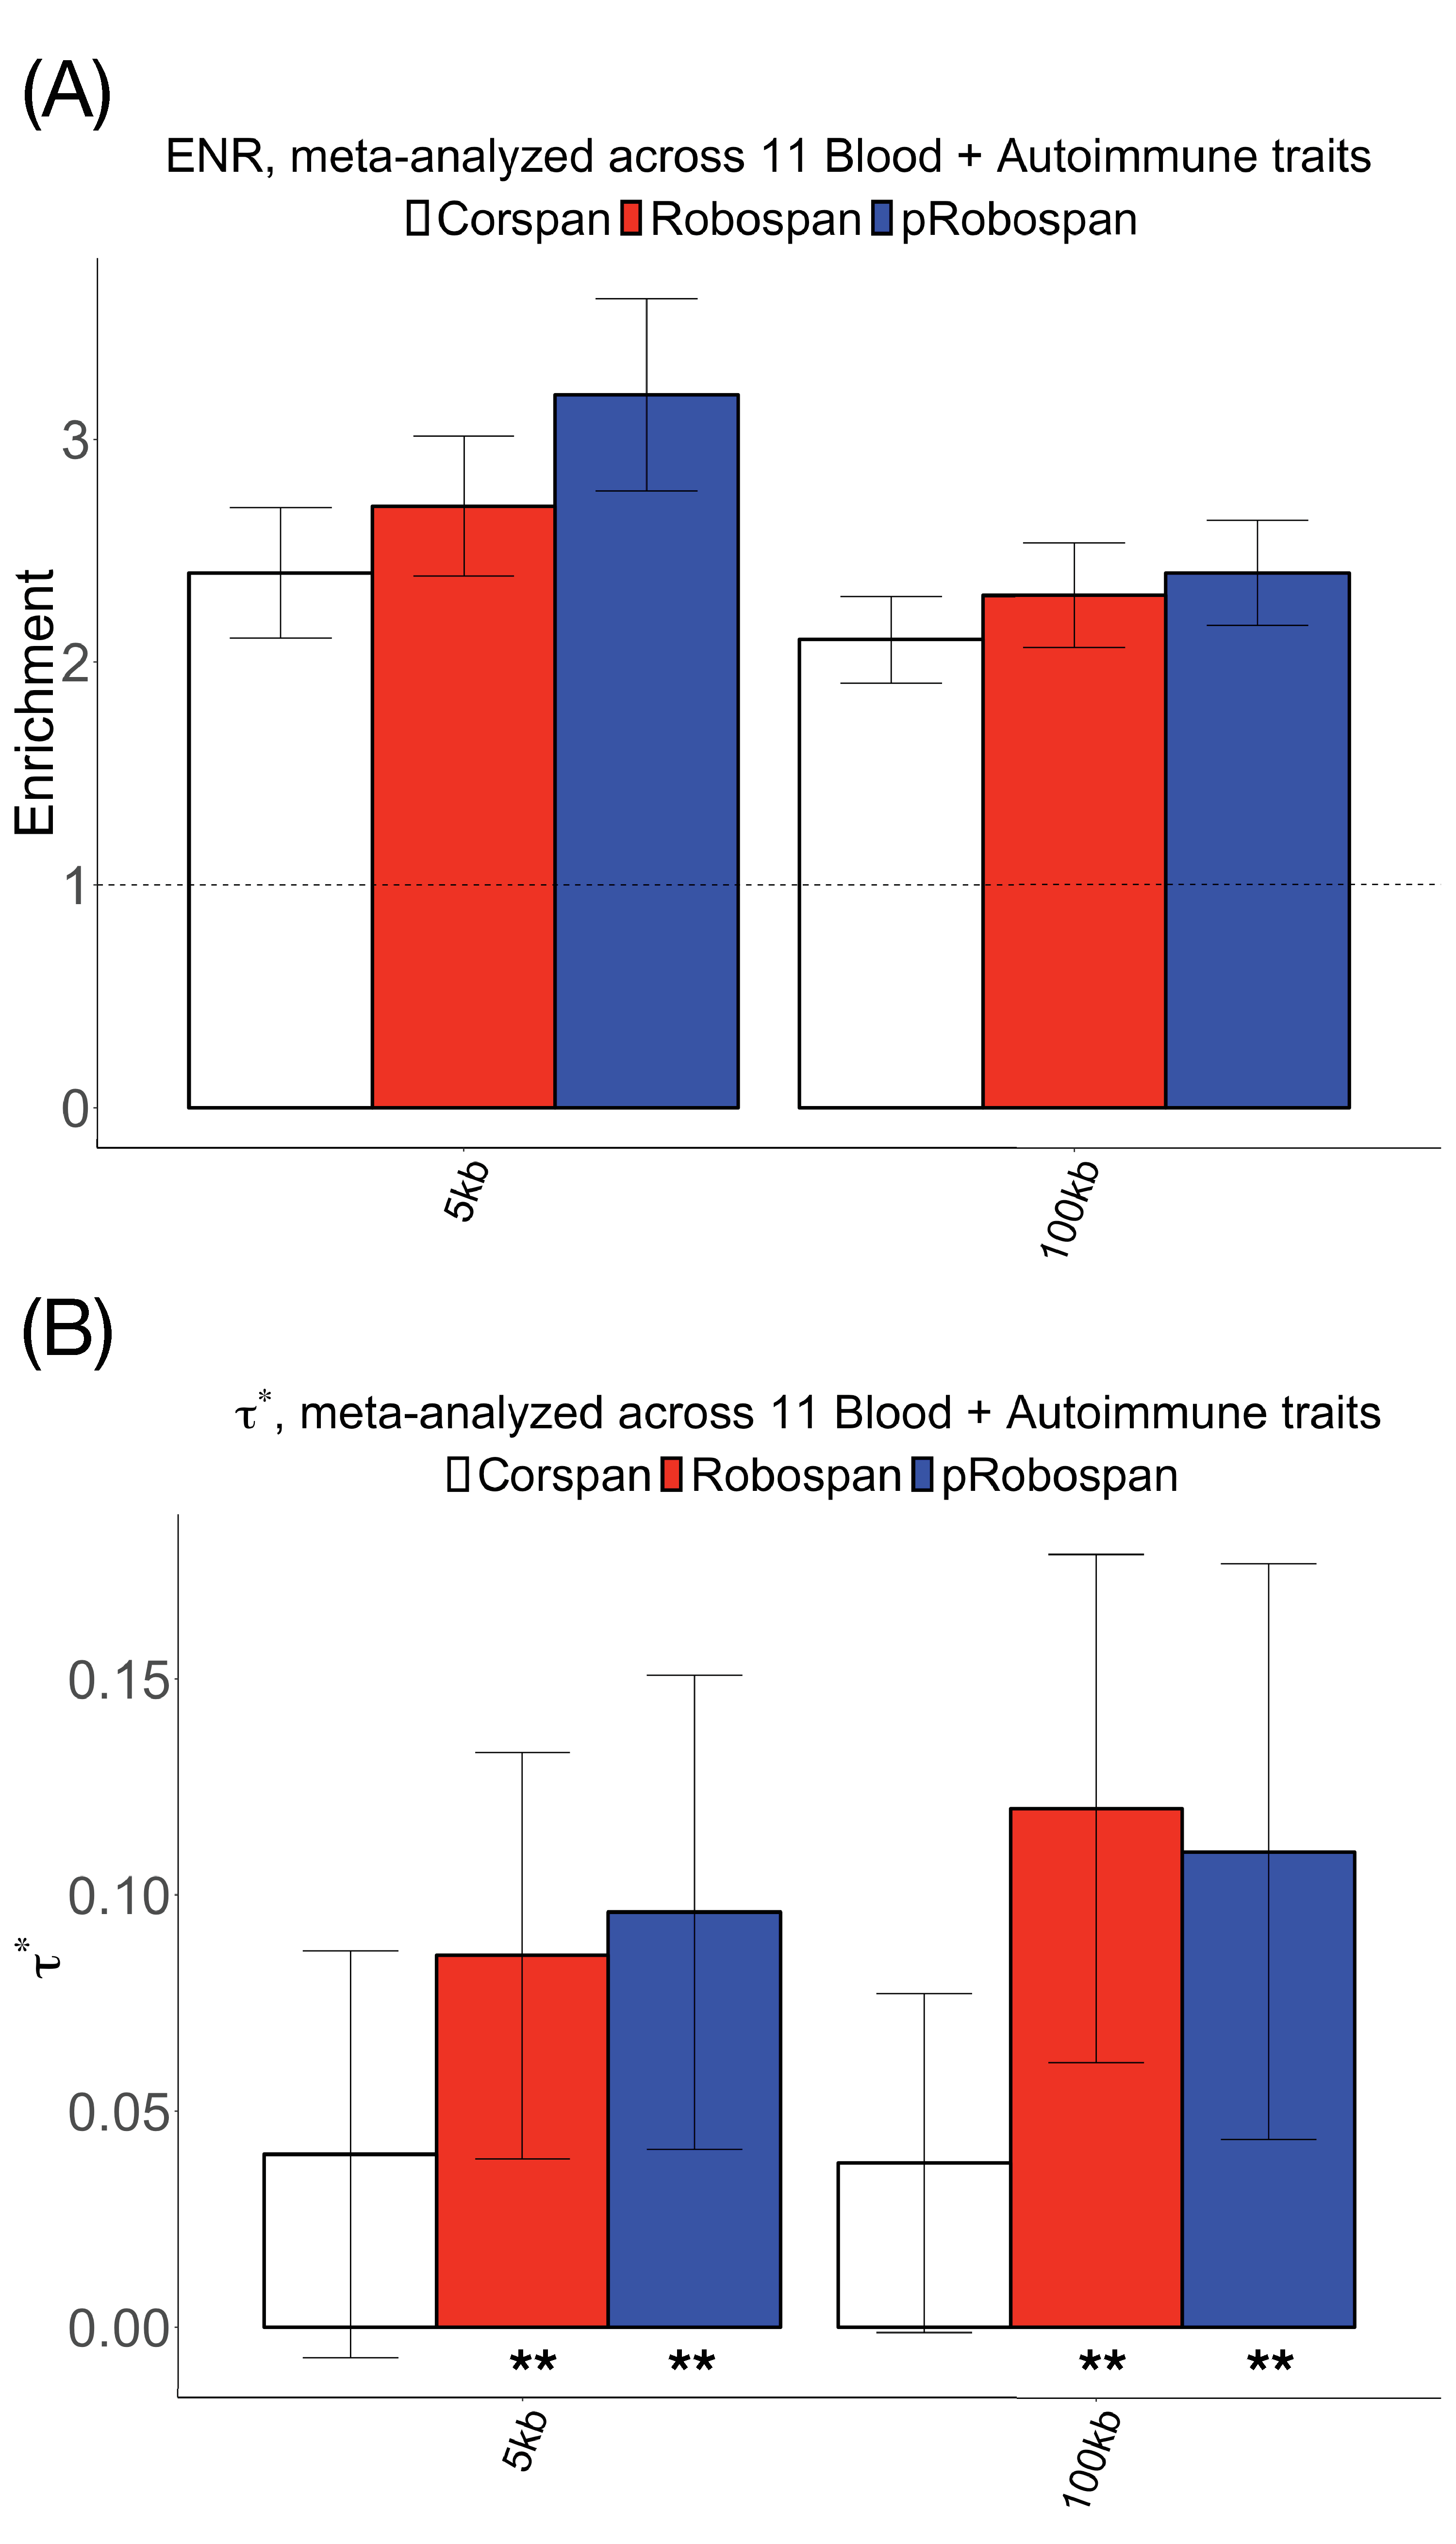
\includegraphics[width=0.4\textwidth]{Figure3_eps.eps}}
\caption{\small {\textbf{Disease informativeness of 5kb and 100kb SNP annotations for \Corspan{}, \Robospan{} and \pRobospan{} gene sets}: (A) Heritability enrichment, conditional on baseline-LD model (v2.1). The base enrichment level is 1. (B) Standardized effect size ($\tau^{\star}$) conditional on baseline-LD model for \Corspan{} (left column, white), \Robospan{} (middle column, red) and \pRobospan{} (right column, blue) gene sets. Results are meta-analyzed across 11 blood and autoimmune traits. ** denotes annotations that are significant after Bonferonni correction ($P < 0.05/8$) where $8$ is the total number of SNP annotations tested. Error bars denote 95$\%$ confidence intervals. Numerical results are reported in Table \ref{tab:Robocov_marginal}.}}
\label{fig:Robocov_marginal}
\end{figure}

For each gene set, we define  SNP-level annotations to test for disease heritability. We define an \emph{annotation} as an assignment of a numeric value to each SNP with minor allele count $\geq$5 in a 1000 Genomes Project European reference panel\cite{1000G2015, Finucane2015}. For each gene set X, we generate two binary SNP-level annotations -- we assign a value of 1 to a SNP if it lies within 5kb or 100kb window upstream and downstream of a gene in the gene set and 0 otherwise; this strategy has been used in several previous works\cite{Finucane2018, Kim2019, deLeeuw2015}.

We assessed the informativeness of SNP annotations for disease heritability by applying stratified LD score regression (S-LDSC)\cite{Finucane2015} conditional on 86 baseline annotations comprising of coding, conserved, epigenomic and LD related annotations (this is called the baseline-LD model; here we use version 2.1\cite{gazal2017}). S-LDSC results were meta-analyzed across 11 relatively independent blood-related traits (5 autoimmune diseases and 6 blood traits (Table \ref{tab:list_blood_traits}).  We considered two S-LDSC metrics for comparison: enrichment and standardized effect size ($\tau^{\star}$) (Supplementary Note).  Enrichment is defined as the proportion of heritability explained by SNPs in an annotation divided by the proportion of SNPs in the annotation\cite{Finucane2015}. Standardized effect size ($\tau^{\star}$) is defined as the proportionate change in per-SNP heritability associated with a 1 standard deviation increase in the value of the annotation, conditional on other annotations included in the model\cite{gazal2017, Hormozdiari2018}; unlike enrichment, $\tau^{\star}$ quantifies effects that are unique to the focal annotation and is a better metric for disease informativeness\cite{dey2019, Kim2019, Finucane2018, Hormozdiari2018}. 

%In our ``marginal'' analyses, we estimated $\tau^{\star}$ for each focal annotation conditional on the 90 baseline-LD$^\star$ annotations. 

All $6$ annotations (5kb and 100kb for the 3 gene scores) were significantly enriched when meta-analyzed across 11 blood and autoimmune traits. However, SNP annotations corresponding to \Robospan{} and \pRobospan{} gene sets showed higher enrichment than  \Corspan{} genes (Figure \ref{fig:Robocov_marginal} and Table \ref{tab:Robocov_marginal}). More importantly, 2 \Robospan{}, 2 \pRobospan{} and 0 \Corspan{} annotations showed significant $\tau^{\star}$ conditional on the baseline-LD annotations after Bonferonni correction (Figure \ref{fig:Robocov_marginal} and Table \ref{tab:Robocov_marginal}). When restricted to the 5 autoimmune traits,  2 \Robospan{}, 0 \pRobospan{} and 0 \Corspan{} SNP annotations showed unique signal (Table \ref{tab:Robocov_marginal_immune}). Even when these annotations were modeled jointly with SEG-Blood\cite{Finucane2018} genes and subjected to forward stepwise elimination similar to ref.\cite{Kim2019, dey2019}, 1 \Robospan{} annotation (100kb) still remains significantly informative, suggesting unique disease information over SEG-Blood genes (Table \ref{tab:Robocov_joint}). 

%obocov{} correlation and partial correlation estimator show higher enrichment and disease informative signal compared to the \Corspan{} gene set constructed similarly from the standard correlation estimator. Additionally, the \Robospan{} gene set shows unique disease information ($\tau^{\star}$) conditional on the specifically expressed gene in blood; this shows that the study of correlation structure of gene expression across tissues adds value over study of expression data alone. 





















